\documentclass{IEEEtran}
\usepackage[T1]{fontenc}
\usepackage[utf8]{inputenc}

\usepackage{cite}
\usepackage{amsmath,amssymb}
\usepackage{graphicx}
\usepackage{booktabs}
\usepackage{array}
\usepackage{xcolor}
\usepackage{url}
\usepackage{tikz}
\usetikzlibrary{positioning,arrows.meta,calc}
\usepackage{pgfplots}
\pgfplotsset{compat=1.17}

\def\BibTeX{{\rm B\kern-.05em{\sc i\kern-.025em b}\kern-.08em
T\kern-.1667em\lower.7ex\hbox{E}\kern-.125emX}}

\newcommand{\code}[1]{\texttt{\small #1}}

\markboth{STUDENT SCIENTIFIC RESEARCH COMMUNICATION, Volume II, 2025}
{[Author] \MakeLowercase{\textit{et al.}}: Multi-Agent Agentic RAG for Safe Automated Checkout}

\begin{document}

\title{Design and Evaluation of Multi-Agent Agentic RAG for Safe Automated Checkout in Multi-Vendor E-Commerce}

\author{ Nguyen Thanh Kiet, Tran Quang Vinh, and Huynh Nam
\thanks{Manuscript submitted [Month Day, Year]. This research received no external funding. The authors declare no conflict of interest.}
\thanks{The authors are with the [Faculty], [University], [City], Vietnam (e-mail: [author1@university.edu.vn]; [author2@university.edu.vn]; [author3@university.edu.vn]).}}

\maketitle

\begin{abstract}
Large-language-model shopping assistants can retrieve products and invoke checkout tools, but an error in routing or consent interpretation can become an unwanted order. This study asks to what extent a code-governed multi-agent agentic retrieval-augmented generation (RAG) architecture can automate checkout while preventing unconfirmed, duplicate, and stale-price orders under model and distributed-system faults. We design a LangGraph supervisor that delegates catalog reasoning to a ProductAgent and transactional work to an OrderAgent. The model may propose an action, but deterministic code authorizes it through a one-time conversational confirmation, a single-use server-side quote, and retry-safe order processing. The implementation is evaluated through the real orchestration and checkout-controller code with scripted models and in-memory service doubles. Across 400 checkout conversations, every target was reached with no write before confirmation. All 23 injected fault cases behaved as specified, and 50 concurrent confirmation requests produced one order in the controller benchmark. At 30\% synthetic interpretation error, the proposed confirmation gate reduced false confirmation from 15.1\% for a model-only policy to 1.0\%, while increasing confirmation recall from 70.2\% to 91.8\%. The results show that transaction safety can be separated from probabilistic language understanding by making the model plan and deterministic code commit.
\end{abstract}

\begin{IEEEkeywords}
Agent safety, agentic retrieval-augmented generation, checkout automation, conversational commerce, idempotency, large language models, multi-agent systems
\end{IEEEkeywords}

% ===========================================================================
\section{Introduction}
\label{sec:introduction}

\IEEEPARstart{R}{etrieval}-augmented generation (RAG) grounds a large language model (LLM) in external evidence before it answers~\cite{lewis2020rag,gao2023ragsurvey}. Agentic RAG extends this pattern: the model decides when to retrieve, evaluates the evidence, and invokes tools~\cite{singh2025agenticrag,yao2023react}. In e-commerce, those tools can search the catalog, modify a cart, and create an order. The capability is useful, but it changes the consequence of an error. A weak recommendation can be ignored; a mistaken interpretation of ``ok, but let me think'' can create a financial transaction.

This work is grounded in a Vietnamese multi-vendor marketplace comprising fourteen services for identity, catalog, inventory, cart, order, payment, wallet, and related functions. Its assistant searches a live catalog and supports checkout in Vietnamese. The implementation exposed a practical safety boundary: the LLM is effective at resolving vague references and product needs, but it is not a reliable authorization mechanism. Tool-using agents still fail many realistic tasks~\cite{yao2024taubench}, prompt-injected content can redirect an agent~\cite{greshake2023injection}, and ordinary networks can repeat timed-out requests~\cite{helland2012idempotence}. Therefore, improving model accuracy alone cannot guarantee that one buyer intention creates exactly one order at the reviewed price.

The paper addresses one research question:

\emph{RQ: To what extent can a code-governed multi-agent Agentic RAG architecture automate checkout while preventing unconfirmed, duplicate, and stale-price orders under LLM interpretation errors and distributed-system faults?}

The unit of study is the path from a proposed cart or checkout action to a persistent order. Product-retrieval quality and end-to-end payment throughput are outside the measured outcome; they are described only where they determine this commit path. The contributions are:

\begin{enumerate}
\item a source-grounded multi-agent architecture in which a supervisor coordinates a catalog-focused ProductAgent and a transaction-focused OrderAgent;
\item a code-governed commit protocol that binds a conversational confirmation to a single-use quote, current catalog state, and an idempotent order request; and
\item a reproducible evaluation on the project code using complete conversations, fault injection, confirmation-policy comparison, and removal of individual safety guards.
\end{enumerate}

% ===========================================================================
\section{Related Work}

\textbf{Agentic retrieval and multi-agent systems.} RAG combines parametric generation with retrieved evidence~\cite{lewis2020rag,gao2023ragsurvey}. Agentic variants add planning, reflection, and adaptive retrieval~\cite{singh2025agenticrag}; ReAct interleaves reasoning and tool actions~\cite{yao2023react}; and AutoGen coordinates specialized agents through conversation~\cite{wu2023autogen}. These methods improve task decomposition and grounding, but they do not by themselves define who is authorized to commit a write.

\textbf{Shopping and acting-agent evaluation.} WebShop evaluates grounded web shopping~\cite{yao2022webshop}, while $\tau$-bench evaluates tool-agent-user interaction over retail and airline databases~\cite{yao2024taubench}. AgentDojo and ToolEmu study prompt injection and risky tool behavior~\cite{debenedetti2024agentdojo,ruan2024toolemu}. These benchmarks reveal that agents are fallible, but their principal outcome is task success or attack resistance rather than the transactional invariant that one explicit confirmation produces at most one current-price order.

\textbf{Distributed transaction safety.} Sagas decompose a long transaction into local steps and compensations~\cite{garciamolina1987sagas}. Idempotency, transactional outboxes, and duplicate-event inboxes address retries and at-least-once delivery in microservices~\cite{helland2012idempotence,richardson2018microservices,kreps2011kafka}. This literature normally assumes that the caller has already been authorized. Our gap lies between the two areas: an uncertain LLM proposes the transaction, while deterministic distributed-system mechanisms must decide whether and how it is committed.

% ===========================================================================
\section{Research Methodology}
\label{sec:method}

\subsection{Research Design and Safety Property}

We followed a design--build--evaluate process. First, we traced the assistant and checkout paths in the project source and identified failures that could create an unintended order. Second, we assigned each probabilistic task to an LLM and each authorization invariant to deterministic code. Third, we implemented the agents and commit protocol. Finally, we tested the proposed method against baselines and guard-removal variants.

The protected property is: \emph{every cart mutation or order must correspond to one unexpired, explicit confirmation from the authenticated buyer, and an order must use the product state and price reviewed by that buyer}. The threat model assumes an honest buyer, an LLM that may misunderstand or fabricate a claim, a client that may forge, delay, or repeat a request, and services that may fail or deliver an event more than once. It does not assume a compromised database or service credential. Table~\ref{tab:threats} maps the threats to code-level controls and evaluation evidence.

\begin{table}[t]
\caption{Threats, Deterministic Controls, and Evidence}
\label{tab:threats}
\centering
\footnotesize
\setlength{\tabcolsep}{3pt}
\begin{tabular}{@{}p{19mm}p{45mm}p{10mm}@{}}
\toprule
Threat & Control & Test \\
\midrule
Unconfirmed or misread action & Pending action; lexical decision followed by a gated model decision & E1--E3 \\
Forged, expired, or replayed confirmation & Random action ID; buyer/session binding; hashed single-use token; expiry & E2 \\
Concurrent or retried request & Atomic quote claim and order idempotency key & E2, E4 \\
Price or stock drift & Canonicalize and re-price immediately before order creation & E2, E4 \\
Model/tool failure or false success claim & No-write fallback and removal of unbacked completion claims & E2 \\
\bottomrule
\end{tabular}
\end{table}

\subsection{Proposed Multi-Agent Agentic RAG Architecture}

The assistant is a Python service built with LangGraph~\cite{langgraph}. Figure~\ref{fig:architecture} shows the implemented control flow. The \code{understand} node receives the buyer message, recent history, visible products, and catalog categories, and asks the LLM for a structured semantic turn. The schema contains at most three tasks, referenced products, constraints, confidence, and a possible interpretation of a pending confirmation. The supervisor resolves expressions such as ``the second one,'' creates a plan, and dispatches one main route. Policy or web-research work may execute as a side branch; a collection barrier joins the results before \code{finalize}. A per-turn call budget prevents an agent loop from issuing unbounded LLM requests.

\begin{figure}[t]
\centering
\resizebox{\columnwidth}{!}{%
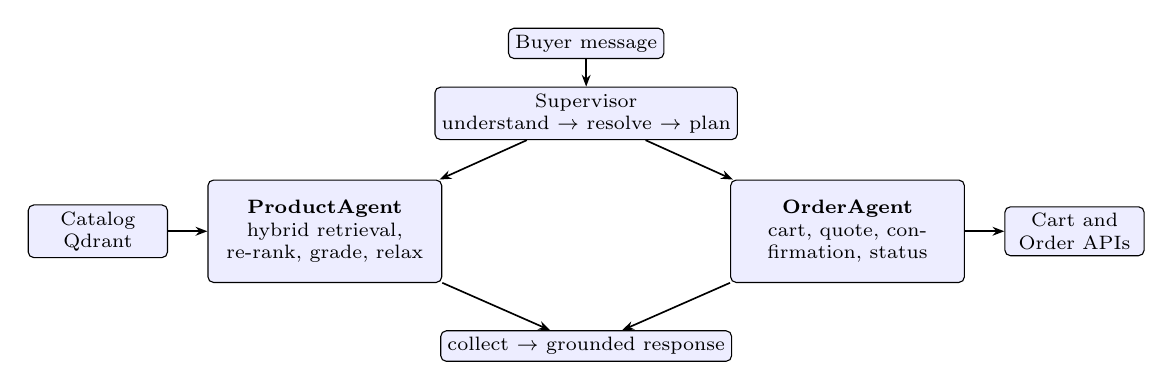
\begin{tikzpicture}[font=\scriptsize,
  box/.style={draw, rounded corners=2pt, fill=blue!7, align=center, inner sep=2.4pt},
  agent/.style={box, text width=28mm, minimum height=13mm},
  arr/.style={-{Stealth[length=1.5mm]}, semithick}]
\node[box] (msg) {Buyer message};
\node[box, below=3.5mm of msg] (sup) {Supervisor\\understand $\rightarrow$ resolve $\rightarrow$ plan};
\node[agent, below left=5mm and -1mm of sup] (prod) {\textbf{ProductAgent}\\hybrid retrieval, re-rank, grade, relax};
\node[agent, below right=5mm and -1mm of sup] (ord) {\textbf{OrderAgent}\\cart, quote, confirmation, status};
\node[box, below=6mm of $(prod.south)!0.5!(ord.south)$] (fin) {collect $\rightarrow$ grounded response};
\node[box, left=5mm of prod, text width=16mm] (cat) {Catalog\\Qdrant};
\node[box, right=5mm of ord, text width=16mm] (svc) {Cart and\\Order APIs};
\draw[arr] (msg) -- (sup);
\draw[arr] (sup) -- (prod);
\draw[arr] (sup) -- (ord);
\draw[arr] (cat) -- (prod);
\draw[arr] (ord) -- (svc);
\draw[arr] (prod) -- (fin);
\draw[arr] (ord) -- (fin);
\end{tikzpicture}
}
\caption{Implemented multi-agent architecture. The LLM supplies semantic plans; only the OrderAgent's deterministic commit path can perform transactional writes.}
\label{fig:architecture}
\end{figure}

The \textbf{ProductAgent} owns read-oriented product work. Product documents are represented by 768-dimensional dense embeddings and BM25 sparse vectors in Qdrant~\cite{qdrant,lee2025geminiembedding,robertson2009bm25}. Dense and lexical rankings are merged by reciprocal rank fusion~\cite{cormack2009rrf}. A local multilingual cross-encoder re-ranks the candidate pool; when enabled, the LLM then grades a short list for semantic needs that catalog fields cannot express. Empty results trigger bounded constraint relaxation and, optionally, web research for product types. Prices and stock are refreshed from marketplace services before display. The ProductAgent has no cart or order write capability.

The \textbf{OrderAgent} owns cart inspection, preparation of cart mutations, checkout, confirmation, and order status. It passes numbered real cart lines or product variants to the model, so a semantic decision must select an existing candidate rather than invent an identifier. Authentication and role checks precede every transaction. Most importantly, preparation and commitment are different operations: preparation records a pending action and returns a summary; it does not write.

\subsection{Code-Governed Commit Protocol}

The protocol in Fig.~\ref{fig:sequence} implements the rule \emph{plan with the model, commit with the code} at three boundaries.

\textit{Layer 1---conversational confirmation.} A proposed mutation becomes a pending action containing a 144-bit random identifier, exact payload, human-readable summary, and 600-s expiry. The assistant commits only when the authenticated session returns the same identifier. Short replies are classified by fixed allow/cancel phrases. Longer replies use the model only if the text begins with an explicit phrase consistent with the model decision. A separate finalizer removes statements claiming that a cart or order changed when no write tool produced evidence. Once an action succeeds or is canceled, its pending state is cleared.

\textit{Layer 2---single-use checkout quote.} Direct checkout is offered only when the request includes a stored address and either cash on delivery or bank transfer; otherwise the assistant opens the ordinary checkout page for the buyer. The order service canonicalizes products, reads current price and stock, validates the address and voucher, and creates a 600-s quote. It returns a 256-bit token once and stores only its SHA-256 digest. The assistant server stores the token inside pending state; it is not shown to the browser or inserted into an LLM prompt. Confirmation checks buyer, chat session, token, status, and expiry. A conditional database update changes the quote from \code{open}/\code{failed} to \code{committing}; only the request that claims it proceeds. Immediately before creating the order, the service canonicalizes all lines again and rejects changed price, stock, or product data. The order request carries \code{Idempotency-Key: checkout:\{quoteId\}}. A committed quote returns its previous order on replay. Wallet checkout is refused until a separate one-time payment approval exists.

\textit{Layer 3---retry-safe payment.} After order creation, payment-related services use a saga with unique debit references, inbox deduplication, and transactional outboxes~\cite{richardson2018microservices}. A failed payment can cancel the order and release stock. This layer completes the production architecture, but the experiments in this paper stop at safe order creation; payment-saga correctness is not claimed as an evaluated result.

\begin{figure}[t]
\centering
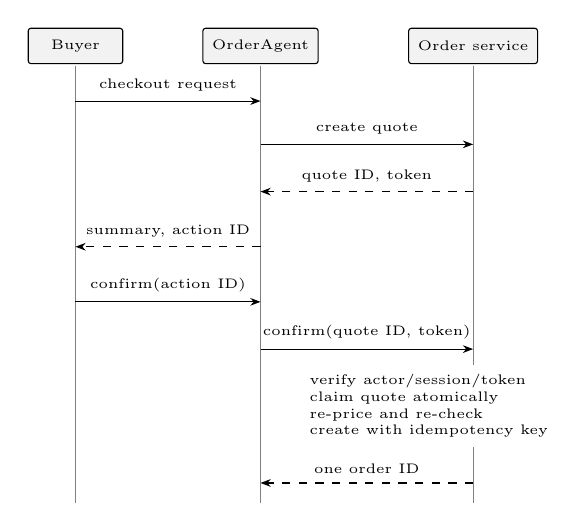
\begin{tikzpicture}[font=\tiny,
  life/.style={draw, fill=gray!10, rounded corners=1pt, minimum width=12mm, minimum height=4.5mm},
  msg/.style={-{Stealth[length=1.3mm]}}, ret/.style={-{Stealth[length=1.3mm]}, dashed}]
\node[life] (u) at (0,0) {Buyer};
\node[life] (a) at (2.35,0) {OrderAgent};
\node[life] (o) at (5.05,0) {Order service};
\foreach \x in {0,2.35,5.05} \draw[gray] (\x,-0.25) -- (\x,-5.8);
\draw[msg] (0,-0.7) -- node[above]{checkout request} (2.35,-0.7);
\draw[msg] (2.35,-1.25) -- node[above]{create quote} (5.05,-1.25);
\draw[ret] (5.05,-1.85) -- node[above]{quote ID, token} (2.35,-1.85);
\draw[ret] (2.35,-2.55) -- node[above]{summary, action ID} (0,-2.55);
\draw[msg] (0,-3.25) -- node[above]{confirm(action ID)} (2.35,-3.25);
\draw[msg] (2.35,-3.85) -- node[above]{confirm(quote ID, token)} (5.05,-3.85);
\node[align=left, anchor=north west, fill=white] at (2.85,-4.05) {verify actor/session/token\\claim quote atomically\\re-price and re-check\\create with idempotency key};
\draw[ret] (5.05,-5.55) -- node[above]{one order ID} (2.35,-5.55);
\end{tikzpicture}
\caption{Binding a conversational action to a server-side quote. The token remains between the assistant server and order service.}
\label{fig:sequence}
\end{figure}

\subsection{Experimental Design}

The evaluation isolates the commit path from general Vietnamese-language accuracy. The test programs import the real agent graph, OrderAgent, confirmation functions, and Node.js checkout controller. The LLM is replaced by a scripted semantic model for E1--E2 and by a controlled noisy classifier for E3. Networked services and persistence are replaced with in-memory doubles that record writes. This design supports repeatable fault injection but does not reproduce production latency or database isolation.

Table~\ref{tab:experiments} summarizes the four experiments. E1 measures functional completion and premature writes. E2 injects authentication, identity, expiry, replay, price, concurrency, model, and downstream-service faults. E3 compares five authorization policies on 46 Vietnamese replies labeled by the authors: 18 confirmations, 10 cancellations, and 18 other replies. For error probability $p$, the noisy model returns the gold label with probability $1-p$ and either wrong label uniformly otherwise; 2,000 trials are run for each $p\in\{0,.1,.2,.3,.4,.5\}$. E4 removes the quote claim, idempotency key, both, or re-pricing in the service double.

\begin{table*}[t]
\caption{Evaluation Plan for the Single Research Question}
\label{tab:experiments}
\centering
\footnotesize
\setlength{\tabcolsep}{4pt}
\begin{tabular}{@{}p{17mm}p{48mm}p{68mm}p{35mm}@{}}
\toprule
Experiment & Input & Intervention and procedure & Measures \\
\midrule
E1 conversation & 200 direct and 200 checkout-page-handoff dialogues & Run the real graph with correct scripted semantic turns; inspect the recorded cart/order writes after each turn & Completion, early writes, orders, model calls, code time \\
E2 faults & 11 agent cases, 12 service cases, 7 response sentences & Inject one fault at a time, including forged/replayed IDs, expiry, price drift, unavailable model, retry, and 2/10/50 concurrent requests & Writes, orders, HTTP status, false success claims \\
E3 policies & 46 labeled replies; 2,000 trials per noise level & Compare direct action (V0), model only (V1), lexical only (V2), proposed two-stage gate (V3), and an in-sample refinement (V4) & False-confirm rate, confirmation recall, model calls \\
E4 guard removal & One quote under concurrency, lost response/retry, and price change & Remove atomic claim, idempotency key, both, or pre-commit re-pricing & Total and stale-price orders \\
\bottomrule
\end{tabular}
\end{table*}

For non-confirming replies $N$ and actual confirmations $Y$, let $FP_N$ be non-confirmations classified as confirm and $TP_Y$ be correctly accepted confirmations. The principal E3 metrics are
\begin{equation}
\mathrm{FCR}=\frac{FP_N}{|N|},\qquad
\mathrm{Recall}=\frac{TP_Y}{|Y|}.
\end{equation}
Lower false-confirm rate (FCR) is safer; higher recall is more convenient. The environment was Windows 11, Python 3.10.0, Node.js 24.5.0, and a LangGraph memory checkpointer. The benchmark scripts, utterances, and raw JSON results are stored in \code{docs/paper/benchmark}.

% ===========================================================================
\section{Experiments and Results}
\label{sec:results}

\subsection{Conversation Completion and Fault Injection}

All 400 E1 conversations reached their specified endpoint (Table~\ref{tab:e1}). Direct mode added a cart line and created one order after two separate confirmations. Handoff mode added the line after confirmation and then opened a populated checkout page, where the normal user interface owns final placement. No run modified the cart or created an order early. Deterministic typed confirmations consumed no LLM call. Median orchestration time was 5.9--8.1~ms per message; this excludes model, network, and database latency and therefore measures code overhead only.

\begin{table}[t]
\caption{E1: Complete Checkout Conversations}
\label{tab:e1}
\centering
\footnotesize
\setlength{\tabcolsep}{4pt}
\begin{tabular}{@{}lcc@{}}
\toprule
Measure & Direct & Handoff \\
\midrule
Runs / messages per run & 200 / 4 & 200 / 3 \\
Goal reached & 200 & 200 \\
Writes / orders before confirmation & 0 / 0 & 0 / 0 \\
Cart writes / orders per run & 1 / 1 & 1 / 0 \\
LLM calls by turn & 1, 0, 1, 0 & 1, 0, 1 \\
Median code time (ms) & 8.1, 6.4, 7.6, 6.4 & 7.4, 5.9, 6.9 \\
\bottomrule
\end{tabular}
\end{table}

All 23 E2 fault cases met their expected write count or status. At the agent boundary, an absent, forged, mismatched, expired, canceled, or unauthenticated action produced no write; replay produced one write; and the explicit-prefix gate rejected a hedged reply even when the model labeled it as confirmation. When the semantic model failed, fallback behavior wrote nothing. The response filter correctly removed four unsupported completion claims and retained three factual/non-committal controls.

At the order-service boundary, wrong token or session was rejected, an expired quote returned HTTP 410, price drift returned 409, and wallet auto-payment required step-up approval. A failed downstream order request followed by retry produced one order. Batches of 2, 10, and 50 concurrent confirmation calls each produced one created order in the controller test double. These tests exercise the conditional-claim logic but not a live database's isolation semantics.

\subsection{Confirmation-Policy Comparison}

Figure~\ref{fig:noise} shows that model-only authorization degrades approximately with the injected interpretation error, while the proposed V3 gate limits the model to replies that are lexically compatible with an explicit decision. At $p=0.3$, V1 accepted 15.1\% of non-confirmations and recalled 70.2\% of confirmations. V3 reduced FCR to 1.0\% and raised recall to 91.8\%, while consulting the model for 0.57 calls per reply. The lexical-only V2 policy had zero false confirmations but only 72.2\% recall because it rejected longer valid replies.

\begin{figure*}[t]
\centering
\pgfplotsset{e3/.style={scale only axis, width=6.2cm, height=3.25cm, xmin=0, xmax=0.5,
  xtick={0,0.1,0.2,0.3,0.4,0.5}, tick label style={font=\footnotesize}, label style={font=\footnotesize},
  legend style={font=\footnotesize, at={(0.5,1.04)}, anchor=south, draw=none, legend columns=-1},
  every axis plot/.append style={thick, mark size=1.6pt}}}
\begin{tikzpicture}
\begin{axis}[e3, ymin=0, ymax=27, xlabel={Synthetic model error $p$}, ylabel={False confirmation (\%)}]
\addplot[red, mark=square*] coordinates {(0,0) (.1,4.9) (.2,9.9) (.3,15.1) (.4,19.8) (.5,25.1)};
\addplot[blue, mark=*] coordinates {(0,0) (.1,.3) (.2,.6) (.3,1.0) (.4,1.4) (.5,1.8)};
\addplot[black!60!green, mark=triangle*, dashed] coordinates {(0,0) (.1,0) (.2,0) (.3,0) (.4,0) (.5,0)};
\legend{V1 model-only,V3 proposed,V2 lexical}
\end{axis}
\end{tikzpicture}\hspace{9mm}%
\begin{tikzpicture}
\begin{axis}[e3, ymin=45, ymax=102, xlabel={Synthetic model error $p$}, ylabel={Confirmation recall (\%)}]
\addplot[red, mark=square*] coordinates {(0,100) (.1,89.8) (.2,80.0) (.3,70.2) (.4,60.1) (.5,49.5)};
\addplot[blue, mark=*] coordinates {(0,100) (.1,97.3) (.2,94.5) (.3,91.8) (.4,89.0) (.5,86.1)};
\addplot[black!60!green, mark=triangle*, dashed] coordinates {(0,72.2) (.1,72.2) (.2,72.2) (.3,72.2) (.4,72.2) (.5,72.2)};
\legend{V1 model-only,V3 proposed,V2 lexical}
\end{axis}
\end{tikzpicture}
\caption{E3 safety and convenience under controlled semantic-label noise. V0 is omitted because its false-confirm rate is 100\%.}
\label{fig:noise}
\end{figure*}

The worst-case classifier always returned ``confirm.'' V1 then committed every reply. V3 still rejected 26 of 28 non-confirmations, but accepted two hedged replies beginning with ``ok,'' for 7.1\% FCR. V4 adds three Vietnamese contrast/deferral markers and rejected both without reducing worst-case confirmation recall. However, V4 was derived from these same 46 utterances; it is a hypothesis for a held-out evaluation, not evidence of general zero-error performance.

\subsection{Guard-Removal Results}

Table~\ref{tab:ablation} identifies the role of each server-side guard. Removing either the claim or key alone did not duplicate concurrent orders in this double because the remaining guard still collapsed the calls. Removing both produced one order per concurrent request. The idempotency key alone prevented a second order when the service had created the first order but its response was lost. Re-pricing alone prevented an order whose catalog price changed after the quote. Therefore, the controls are complementary rather than redundant: the claim manages simultaneous ownership of a quote, the key spans downstream retries, and re-pricing binds authorization to current state.

\begin{table}[t]
\caption{E4: Orders After Removing a Guard}
\label{tab:ablation}
\centering
\footnotesize
\setlength{\tabcolsep}{3.5pt}
\begin{tabular}{@{}lccc@{}}
\toprule
Version & Concurrent 2/10/50 & Retry & Stale price \\
\midrule
Full protocol & 1 / 1 / 1 & 1 & 0 \\
No atomic claim & 1 / 1 / 1 & 1 & 0 \\
No idempotency key & 1 / 1 / 1 & \textbf{2} & 0 \\
No claim or key & \textbf{2 / 10 / 50} & \textbf{2} & 0 \\
No re-pricing & 1 / 1 / 1 & 1 & \textbf{1} \\
\bottomrule
\end{tabular}
\end{table}

\subsection{Answer to the Research Question}

Within the evaluated commit boundary, the architecture automated both direct and user-interface-handoff checkout without early writes, contained injected identity, expiry, replay, retry, concurrency, price, and model faults, and depended substantially less on the model for consent interpretation. The strongest quantitative evidence is the reduction from 15.1\% to 1.0\% FCR at $p=0.3$ together with higher recall, and the ablation evidence that duplicate and stale-price orders reappear when their corresponding deterministic guards are removed. The answer is therefore qualified: code governance was effective in this implementation and test model, but it is not yet a production-scale or population-level guarantee.

% ===========================================================================
\section{Discussion}

\subsection{Implications}

The main design implication is a separation of authority. LLMs are well suited to mapping Vietnamese language to structured candidates, resolving references, and judging soft product preferences. They are poorly suited to being the final authority for a write. The commit capability should instead require evidence that a model cannot invent: an authenticated actor, a pending action created by the server, an exact identifier, an unexpired token, and current marketplace state. This separation also improves diagnosis. A false-confirmation metric evaluates the conversational gate; concurrency and retry experiments evaluate the service protocol; neither is hidden inside a single end-to-end success score.

The multi-agent split is functional rather than merely role-based. The ProductAgent is restricted to retrieval and grounded read operations, whereas the OrderAgent is the only component that prepares transactional state. This creates a smaller auditable surface than giving every agent generic tool access. The default checkout-page handoff is also a useful safety policy: conversational direct checkout is an optimization available only when the required address and payment conditions are already satisfied.

\subsection{Limitations and Threats to Validity}

\textbf{Construct validity.} E1--E2 use scripted semantic turns, so they test commit correctness rather than open-ended Vietnamese understanding. E3 simulates independent label noise; real errors are correlated with phrasing, context, and model family. The 46 replies were written and labeled by the authors, and V4 was tuned in-sample.

\textbf{Internal validity.} The scripts import the production graph and controller, but replace databases and remote services. The concurrency double models the conditional update atomically; a live deployment still requires an integration test against the configured database and isolation level. Timing excludes model, network, and storage latency. The ablation switches exist only in the service double so that unsafe variants are not shipped.

\textbf{External validity.} Results come from one Vietnamese marketplace and may not transfer to other languages, payment regulations, or user populations. No human participants or personal data were used, and no usability study was conducted. Product-search relevance, prompt-injection resistance, and the payment saga require separate measurements. Future work will evaluate V3/V4 on held-out naturally collected replies, run a real LLM with simulated buyers, execute concurrency and crash-recovery tests against production-equivalent databases, and measure catalog retrieval on labeled Vietnamese queries.

% ===========================================================================
\section{Conclusion}

This paper investigated one question: whether Multi-Agent Agentic RAG can automate checkout without allowing probabilistic language interpretation to authorize an unsafe order. The proposed architecture assigns catalog reasoning to a ProductAgent, transaction preparation to an OrderAgent, and final authority to deterministic confirmation, quote, re-pricing, and idempotency controls. In code-level experiments, 400 conversations completed without early writes, 23 injected faults produced their expected safe outcomes, and the proposed confirmation gate reduced false confirmation from 15.1\% to 1.0\% at 30\% synthetic model error while improving recall. Guard removal showed why the atomic claim, idempotency key, and price re-check are each necessary. These results support a practical principle for transactional agents: use the model to interpret and plan, but require code-held evidence to commit.

% ===========================================================================


% ===========================================================================
\begin{thebibliography}{00}
\bibitem{lewis2020rag} P. Lewis, E. Perez, A. Piktus, F. Petroni, V. Karpukhin, N. Goyal, H. K\"{u}ttler, M. Lewis, W.-t. Yih, T. Rockt\"{a}schel, S. Riedel, and D. Kiela, ``Retrieval-augmented generation for knowledge-intensive NLP tasks,'' in \textit{Proc. Adv. Neural Inf. Process. Syst. (NeurIPS)}, vol. 33, 2020.
\bibitem{gao2023ragsurvey} Y. Gao, Y. Xiong, X. Gao, K. Jia, J. Pan, Y. Bi, Y. Dai, J. Sun, M. Wang, and H. Wang, ``Retrieval-augmented generation for large language models: A survey,'' 2023, arXiv:2312.10997.
\bibitem{singh2025agenticrag} A. Singh, A. Ehtesham, S. Kumar, T. T. Khoei, and A. V. Vasilakos, ``Agentic retrieval-augmented generation: A survey on agentic RAG,'' 2025, arXiv:2501.09136.
\bibitem{yao2023react} S. Yao, J. Zhao, D. Yu, N. Du, I. Shafran, K. Narasimhan, and Y. Cao, ``ReAct: Synergizing reasoning and acting in language models,'' in \textit{Proc. Int. Conf. Learn. Represent. (ICLR)}, 2023.
\bibitem{wu2023autogen} Q. Wu, G. Bansal, J. Zhang, \textit{et al.}, ``AutoGen: Enabling next-gen LLM applications via multi-agent conversation,'' 2023, arXiv:2308.08155.
\bibitem{yao2022webshop} S. Yao, H. Chen, J. Yang, and K. Narasimhan, ``WebShop: Towards scalable real-world web interaction with grounded language agents,'' in \textit{Proc. Adv. Neural Inf. Process. Syst. (NeurIPS)}, vol. 35, 2022.
\bibitem{yao2024taubench} S. Yao, N. Shinn, P. Razavi, and K. Narasimhan, ``$\tau$-bench: A benchmark for tool-agent-user interaction in real-world domains,'' 2024, arXiv:2406.12045.
\bibitem{greshake2023injection} K. Greshake, S. Abdelnabi, S. Mishra, C. Endres, T. Holz, and M. Fritz, ``Not what you've signed up for: Compromising real-world LLM-integrated applications with indirect prompt injection,'' in \textit{Proc. ACM Workshop Artif. Intell. Secur.}, 2023, pp. 79--90.
\bibitem{debenedetti2024agentdojo} E. Debenedetti, J. Zhang, M. Balunovi\'{c}, L. Beurer-Kellner, M. Fischer, and F. Tram\`{e}r, ``AgentDojo: A dynamic environment to evaluate prompt injection attacks and defenses for LLM agents,'' in \textit{Proc. NeurIPS Datasets Benchmarks Track}, 2024.
\bibitem{ruan2024toolemu} Y. Ruan, H. Dong, A. Wang, \textit{et al.}, ``Identifying the risks of LM agents with an LM-emulated sandbox,'' in \textit{Proc. Int. Conf. Learn. Represent. (ICLR)}, 2024.
\bibitem{garciamolina1987sagas} H. Garcia-Molina and K. Salem, ``Sagas,'' in \textit{Proc. ACM SIGMOD Int. Conf. Manage. Data}, 1987, pp. 249--259.
\bibitem{helland2012idempotence} P. Helland, ``Idempotence is not a medical condition,'' \textit{ACM Queue}, vol. 10, no. 4, p. 30, Apr. 2012.
\bibitem{richardson2018microservices} C. Richardson, \textit{Microservices Patterns: With Examples in Java}. Shelter Island, NY, USA: Manning, 2018.
\bibitem{kreps2011kafka} J. Kreps, N. Narkhede, and J. Rao, ``Kafka: A distributed messaging system for log processing,'' in \textit{Proc. 6th Int. Workshop Netw. Meets Databases}, 2011.
\bibitem{langgraph} LangChain, ``LangGraph: Build resilient language agents as graphs,'' Software. [Online]. Available: \url{https://github.com/langchain-ai/langgraph}. Accessed: Nov. 8, 2026.
\bibitem{qdrant} Qdrant, ``Qdrant: Vector search engine and vector database,'' Software. [Online]. Available: \url{https://github.com/qdrant/qdrant}. Accessed: Nov. 8, 2026.
\bibitem{lee2025geminiembedding} J. Lee, F. Chen, S. Dua, D. Cer, M. Shanbhogue, I. Naim, \textit{et al.}, ``Gemini Embedding: Generalizable embeddings from Gemini,'' 2025, arXiv:2503.07891.
\bibitem{robertson2009bm25} S. Robertson and H. Zaragoza, ``The probabilistic relevance framework: BM25 and beyond,'' \textit{Found. Trends Inf. Retr.}, vol. 3, no. 4, pp. 333--389, 2009.
\bibitem{cormack2009rrf} G. V. Cormack, C. L. A. Clarke, and S. B\"{u}ttcher, ``Reciprocal rank fusion outperforms Condorcet and individual rank learning methods,'' in \textit{Proc. ACM SIGIR}, 2009, pp. 758--759.
\end{thebibliography}

\end{document}
